% !TEX root = ../VLDB-2026-DAGSmith-Dependency-Aware-Rewriting-for-dbt-Style-SQL-Pipelines.tex
\section{Approach}
\label{dag:sec:approach}

% Required preamble (in main.tex):
%   \usepackage{tikz}
% This file loads its own TikZ libraries below, so no \usetikzlibrary
% is needed in main.tex on its account.

\usetikzlibrary{arrows.meta, positioning, shapes.geometric, fit, calc}

\begin{figure*}[t]
\inv
\centering
\resizebox{\textwidth}{!}{%
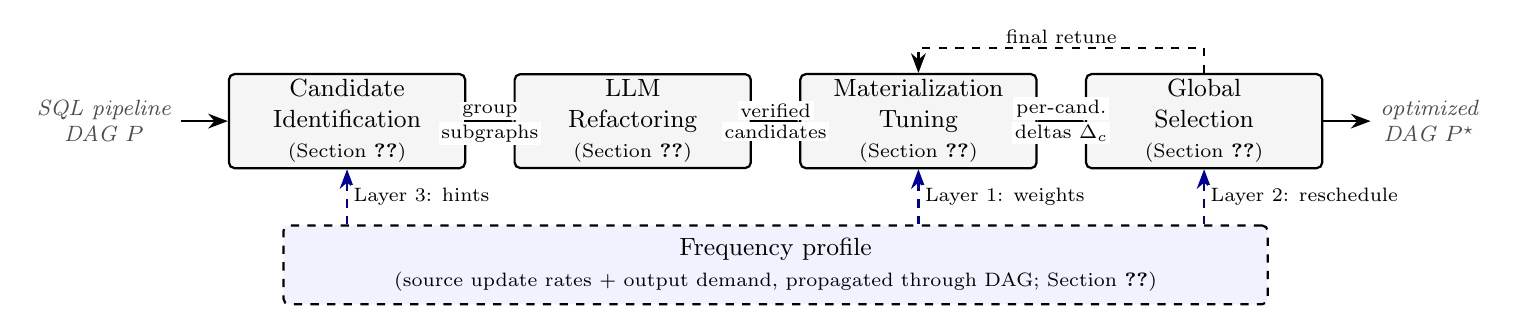
\begin{tikzpicture}[
    font=\small,
    node distance=4mm and 6mm,
    stage/.style={
        draw, rounded corners=2pt, thick,
        minimum height=10mm, minimum width=30mm,
        align=center, fill=black!4,
        inner sep=2pt
    },
    freqstage/.style={
        draw, rounded corners=2pt, thick, dashed,
        minimum height=4mm, minimum width=28mm,
        align=center, fill=blue!5,
        inner sep=2pt
    },
    io/.style={
        align=center, font=\footnotesize\itshape, text=black!70
    },
    arrow/.style={
        -{Stealth[length=2.5mm]}, thick
    },
    freqarrow/.style={
        -{Stealth[length=2.5mm]}, thick, dashed, draw=blue!60!black
    },
    arrowlabel/.style={
        font=\scriptsize, midway, fill=white, inner sep=1pt
    }
]

% --- input ---
\node[io] (input) {SQL pipeline\\DAG $P$};

% --- four pipeline stages, left to right ---
\node[stage, right=of input] (s1) {Candidate\\Identification\\\scriptsize(Section~\ref{dag:sec:candidate-identification})};
\node[stage, right=of s1]    (s2) {LLM\\Refactoring\\\scriptsize(Section~\ref{dag:sec:llm-refactoring})};
\node[stage, right=of s2]    (s3) {Materialization\\Tuning\\\scriptsize(Section~\ref{dag:sec:materialization})};
\node[stage, right=of s3]    (s4) {Global\\Selection\\\scriptsize(Section~\ref{dag:sec:materialization})};

% --- output ---
\node[io, right=of s4] (output) {optimized\\DAG $P^\star$};

% --- main pipeline arrows with artifact labels ---
\draw[arrow] (input) -- (s1);
\draw[arrow] (s1) -- node[arrowlabel, above]{group} node[arrowlabel, below]{subgraphs} (s2);
\draw[arrow] (s2) -- node[arrowlabel, above]{verified} node[arrowlabel, below]{candidates} (s3);
\draw[arrow] (s3) -- node[arrowlabel, above]{per-cand.} node[arrowlabel, below]{deltas $\Delta_c$} (s4);
\draw[arrow] (s4) -- (output);

% --- frequency profile band: one wide box spanning under stages s1-s4 ---
\node[freqstage, below=2mm of s2.south,
      minimum width=125mm, minimum height=10mm,
      anchor=north] (fband)
  at ($(s1.south west)!0.5!(s4.south east) + (0,-5mm)$)
  {Frequency profile\\\scriptsize(source update rates + output demand,
   propagated through DAG; Section~\ref{dag:sec:frequency})};

% Frequency arrows: profile feeds the three stages it touches, each labeled by layer
\draw[freqarrow] (fband.north -| s1.south) -- (s1.south)
  node[arrowlabel, right=1pt, fill=white]{\scriptsize Layer 3: hints};
\draw[freqarrow] (fband.north -| s3.south) -- (s3.south)
  node[arrowlabel, right=1pt, fill=white]{\scriptsize Layer 1: weights};
\draw[freqarrow] (fband.north -| s4.south) -- (s4.south)
  node[arrowlabel, right=1pt, fill=white]{\scriptsize Layer 2: reschedule};

% Final tuning loop-back: flat elbow (saves the vertical space the arc used)
\coordinate (rtlvl) at ($(s4.north)+(0,3.2mm)$);
\draw[arrow, dashed] (s4.north) -- (s4.north|-rtlvl)
  -- node[arrowlabel, above, fill=white]{final retune} (s3.north|-rtlvl)
  -- (s3.north);;

\end{tikzpicture}%
}
% \inv
\caption{End-to-end pipeline of \dagsmith. The top row shows the four main stages and the artifacts that flow between them; after global selection, a final materialization pass retunes the combined DAG. The dashed band underneath is the frequency dimension (Section~\ref{dag:sec:frequency}): a single frequency profile feeds three of the four stages, contributing structural splitting hints, cost weights for materialization tuning, and schedule corrections at selection. }
\label{dag:fig:pipeline}
\inv
\end{figure*}

%\linc{IMPORTANT: We need to double check all the references to the ``opportunites'' in this section. It seems that Barzan has removed the numbered opportunites in Section 2.2, but we still have the six ``optimizations''in Section 1. So we can probably just reference these \textbf{optimizations} by number from Section 1. But double check everything to make sure that the numbers are consistent.}
%\dagjie{Fixed, several revisions have been implemented throughout section 3.}


%\linc{Okay in general, I think this section has way too many implementation details and less intuitive lessons. The purpose of a paper is not to document every details of the implementation so that others will recreate every single step. You'll have your code released and they can reference your code anyway. Rather, the purpose is do convery what are the key technical challenges to solve this problem, (intuitively) what are our solutions to solve these challenges and why we choose these solutions, and what lessons did we learn. Implementaiton details are helpful only if we have the space and if that supports our argument for the solution. But having too many can be distracting. I also think having 5 subsections (components) are a bit too many. I would suggest having only 3-4 subsections. (I think earlier you wrote there are 3 optimization dimensions? That might be a good breakdown for the subsections. It seems that in the ablation study you only categorize three optimizations anyway.) And within each subsection, you start with what technical challenges you're going to solve (and why such challenges exist in our problem), and intuitively how your solution works (and why it solves the challenges). A figure illustrating the sollution would be a plus. Then, you go into a little bit of details to just have the audience have a slighly deeper understanding. You can take a look at other papers (or even your previous papers) to see how long this should be. Readers/Reviewers won't appreciate if you add too many details and they couldn't easily get the big picture.}

\dagsmith{} implements the six optimization opportunities introduced in Section~\ref{dag:sec:dependencies-as-signals} through three interacting implementation dimensions: graph refactoring, materialization tuning, and refresh-frequency tuning. Graph refactoring realizes dependency-edge simplification, non-local semantic reuse, downstream-aware pruning, and pipeline-aware work placement; materialization tuning realizes rewrite-materialization co-optimization by scoring each rewrite under its best table-or-view choices; and refresh-frequency tuning realizes frequency-aware optimization by aligning execution with both input-change rates and output-consumption rates. Global selection is a separate orchestration step that chooses a compatible subset of the candidates produced by these dimensions. Because our implementation and evaluation use dbt projects, this section uses \emph{model} to denote a SQL transformation node.
% \linc{If I remember correctly, Table 1 is just used for us to reference internally to make the terminology consistent, and we'll delete that eventually? If you're unsure, you can probably coordinate with Barzan.}
These dimensions are coupled: the best choice along one depends on the others, so they should not be optimized independently. We quantify these interactions with an ablation study in Section~\ref{dag:sec:eval-attribution}.

% The benefit of a refactoring depends on which nodes are materialized, the best materialization configuration depends on the structure of the DAG, and both depend on how often each node executes. A pipeline with hundreds or thousands of models admits an enormous space of candidate refactorings, materialization assignments, and refresh schedules; exhaustive search is infeasible, and optimizing the three dimensions in separate passes misses these interactions and produces decisions that conflict at the boundaries.

%\linc{I think we need to reference Figure 5 at the beginning of this paragraph}
\dagsmith{} realizes these dimensions in the pipeline of Figure~\ref{dag:fig:pipeline}. Cheap structural analyses first scan the whole DAG and rank model groups by a fingerprint-based score that estimates the benefit of refactoring them jointly (Section~\ref{dag:sec:candidate-identification}). The top-ranked groups are passed to an LLM, which reasons over each region and proposes one or more concrete refactorings (Section~\ref{dag:sec:llm-refactoring}). 
The structural analyses decide where in the DAG to refactor; the LLM decides what refactoring to perform.
%\linc{Since we mentioned LLM, I think we need to add one sentence to talk about the correctness guarantee. Otherwise, I think that would be the first question that the reviewer raises.}
Every refactoring is adopted only after it passes data-backed equivalence checks run against the project's real data: a rewrite is rejected whenever its output diverges from the original's, so acceptance rests on observed agreement rather than the LLM's own assurance.
A refactoring's benefit depends on how its nodes are materialized, so \dagsmith{} tunes each candidate's materialization with a learned cost model and selects a compatible subset to adopt (Section~\ref{dag:sec:materialization}). The frequency-aware optimization affects all these stages (Section~\ref{dag:sec:frequency}): it reweights the cost-driven decisions, removes refreshes that recompute unchanged data, and contributes structural splitting candidates using a frequency profile that combines source update rates with downstream output demand.





% % Required preamble (add to main.tex if not already there):
% % \usepackage{algorithm}
% % \usepackage{algpseudocode}

% \begin{algorithm}[t]
% \caption{\dagsmith{} optimization pipeline.}
% \label{dag:alg:pipeline}
% \begin{algorithmic}[1]
% \Require SQL pipeline DAG $P$, frequency profile $\Phi$
% \Ensure optimized DAG $P^\star$
% \State $f \gets \textsc{PropagateFrequencies}(P, \Phi)$
% \State $\mathcal{G} \gets \textsc{ReuseAnalysis}(P) \cup \textsc{PruneAnalysis}(P)$
% \Statex \hspace{3.6em} $\cup\ \textsc{FrequencySplitHints}(P, f)$ \Comment{\S\ref{dag:sec:candidate-identification}}
% \State $\mathcal{C} \gets \textsc{LLMRefactor}(\mathcal{G}, P)$ \Comment{\S\ref{dag:sec:llm-refactoring}}
% \State $\delta_{\text{orig}} \gets \textsc{MaterializationTune}(P, f)$ \Comment{\S\ref{dag:sec:materialization}}
% \ForAll{$c \in \mathcal{C}$}
%   \State $P_c \gets \textsc{Apply}(P, c)$
%   \State $\Delta_c \gets \delta_{\text{orig}} - \textsc{MaterializationTune}(P_c, f)$
% \EndFor
% \State $H \gets \textsc{ConflictGraph}(\mathcal{C})$
% \State $\mathcal{C}^\star \gets \textsc{SelectILP}(\mathcal{C}, \{\Delta_c\}, H)$ \Comment{\S\ref{dag:sec:materialization}}
% \State $P^\star \gets \textsc{Apply}(P, \mathcal{C}^\star)$
% \State $\textsc{MaterializationTune}(P^\star, f)$ \Comment{final retune}
% \State \Return $\textsc{ReconcileSchedule}(P^\star, f)$ \Comment{\S\ref{dag:sec:frequency}}
% \end{algorithmic}
% \end{algorithm}


\subsection{Candidate Identification}
\label{dag:sec:candidate-identification}

%\linc{I don't think we have established why we want to use LLM for refactoring yet. So I think either you have to establish that here, or just talk about refactoring is costly in general, without specifically emphasizing LLMs.}
Candidate identification finds where in the DAG  the four graph-refactoring optimizations from Section~\ref{dag:sec:dependencies-as-signals} are worth pursuing.
\dagsmith{} confines the refactoring to small, bounded regions rather than the whole project to ensure  the reasoning complexity over these interdependent models is tractable.
Since many regions may not be worth refactoring, \dagsmith{} first scans the  DAG with cheap structural analyses that rank regions by likely benefit, reserving the expensive refactoring step (Section~\ref{dag:sec:llm-refactoring}) for the few that pay off.

%\linc{Before getting into all the details below, I think it would be good to have one paragraph to discuss intuitively how your analysis works and what it achieves (if you can pair that with a figure, that's even better). The rest of this subsection is just implementation details. If intuitively the method makes sense, we would be good. We can either keep the details below or just condense them if we're short on space.}
The analysis must decide when two models perform the same expensive work, and the natural ways of testing for this fall short.
For example, matching on SQL text fails when the same logic is written differently. Matching on plan structure goes further—multi-query optimization and view-matching are already invariant to join order, predicate order, and aliasing—but it reasons about one compiled query at a time and treats a referenced model as an opaque input.
Therefore, it cannot recognize work shared across model boundaries. Figure~\ref{dag:fig:dataflow-grouping} shows the problem: Models A and B compute the same join, but Model A filters its input inline while Model B reads the already-filtered input from a sibling model it references. On the compiled SQL, a plan-subtree matcher therefore sees two unrelated trees over different tables.

To address such challenges, DAGSmith matches on the operation each model computes via dataflow analysis, resolving references so that a model boundary no longer hides shared work, and reduces the two to a single reuse candidate, which the LLM and a data-backed equivalence check confirm is safe to share. It further performs two analyses: reuse finds repeated expensive work to share (non-local semantic reuse), and prune finds work that no downstream model consumes or that runs too early (dependency-edge simplification, downstream-aware pruning, and pipeline-aware work placement). Only the highest-scoring regions are passed to the LLM.

%At its core the analysis must decide when two models do the same expensive work, and the obvious tests miss real cases. Matching SQL text fails on any rephrasing. Matching plan structure is stronger, since multi-query optimization and view-matching already handle join order, predicate order, and aliasing, but it is keyed on the shape of one compiled query and treats a referenced model as an opaque input, so it misses work shared across model boundaries. In Figure~\ref{dag:fig:dataflow-grouping}, Models A and B compute the same join, but Model A filters its input inline while Model B reads the already-filtered input from a sibling model it references, so on the compiled SQL a plan-subtree matcher sees two different trees over different tables.
%\dagsmith{} instead matches on the operation each model computes, resolving references so that a model boundary does not hide shared work, and reduces the two to a single reuse candidate that the LLM and an equivalence check later confirm is safe to share. Two analyses work this way: \emph{reuse} finds repeated expensive work to share (opportunity~(2)), and \emph{prune} finds work that no downstream model consumes or that runs too early (opportunities~(1), (3), and~(4)). Only the highest-scoring regions go to the LLM.

\begin{figure}[tb]
% \inv
\centering
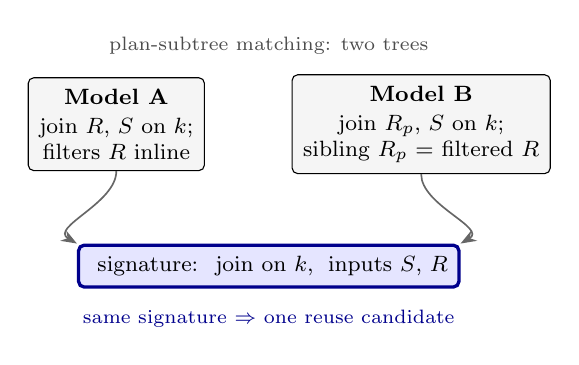
\begin{tikzpicture}[
  font=\small,
  >={Stealth[length=2mm]},
  q/.style={draw, rounded corners=2pt, align=center, fill=black!4, inner sep=4pt, font=\footnotesize},
  canon/.style={draw=blue!55!black, very thick, rounded corners=2pt, align=center, fill=blue!10, inner sep=4pt, font=\footnotesize},
  arr/.style={->, semithick, draw=black!60},
  lbl/.style={font=\scriptsize, text=black!70}
]
\node[q] (A) {\textbf{Model A}\\[1pt]join $R$, $S$ on $k$;\\ filters $R$ inline};
\node[q, right=11mm of A] (B) {\textbf{Model B}\\[1pt]join $R_p$, $S$ on $k$;\\ sibling $R_p$ = filtered $R$};
% plan-matcher verdict above the boxes
\node[lbl, anchor=south] (top) at ($(A.north)!0.5!(B.north)+(0,1.5mm)$)
  {plan-subtree matching: two trees};
% signature below, leaving room for the curved arrows
\node[canon, anchor=north] (C) at ($(A.south)!0.5!(B.south)+(0,-9mm)$)
  {\dagsmith{} signature:\; join on $k$,\; inputs $S$, $R$};
\draw[arr] (A.south) to[out=-90, in=150] (C.north west);
\draw[arr] (B.south) to[out=-90, in=30]  (C.north east);
\node[lbl, text=blue!55!black, below=1.5mm of C] {same signature $\Rightarrow$ one reuse candidate};
\end{tikzpicture}
% \inv
\caption{
Candidate identification discovers shared computation across models based on dataflow, not plan shape.
Models A and B compute the same join on $k$, but Model A filters $R$ inline while Model B reads the already-filtered $R$ from a sibling model $R_p$; on the compiled SQL the two are different trees over different tables, while \dagsmith{} resolves the reference and reduces both to one signature and a single reuse candidate.}
\label{dag:fig:dataflow-grouping}
\inv
\end{figure}

\head{Dataflow representation}
Both analyses run on a \emph{dataflow representation} rather than on SQL text: \dagsmith{} compiles each model into a tree of typed operators and resolves every column and \code{ref()} back through the models that produced it. Figure~\ref{dag:fig:dataflow-grouping} shows why this is needed. Model B reads the sibling $R_p$, so at the SQL level its input is an opaque table name; resolving the reference substitutes $R_p$'s definition, the filtered $R$, and reconstructs the join B actually computes over $R$ and $S$. Model A reaches the same operation by filtering $R$ inline.
The two resolved trees coincide even though the \code{ref()} boundary hides the correspondence in the source, so the analyses can compare models by what they compute rather than by how the SQL is split across the DAG.

\head{Reuse analysis}
Reuse analysis summarizes each model's dataflow representation by a \emph{signature}: its expensive operations (joins and group-by aggregations), the keys they operate on, and their resolved inputs. Models whose signatures match are grouped into one \emph{reuse candidate}; the candidates are scored and ranked by the heuristic described below.
% Reuse analysis summarizes each model's dataflow representation by a \emph{signature}: its expensive operations (joins and group-by aggregations), the keys they operate on, and their resolved inputs. Models whose signatures match are grouped into one candidate and \textit{scored} by the cost of the shared operation and the number of models that share it. \linc{How the score is defined is still slightly vague. Can you be a bit more specific? Edit: see the comment at the end of this subsection first.} A high score is a \emph{targeting signal} that marks where the LLM should look.

\head{Prune analysis}
Prune analysis targets joins in two forms. A \emph{redundant} join produces a result no downstream model consumes, confirmed by tracing column lineage from the leaf models, and can be removed outright or, when it is a semi-join whose filter is already derivable from the probed relation, collapsed to a predicate. A \emph{mistimed} join is correct but computed too early, inflating an expensive downstream operation whose result does not depend on it; pushing it past that operation avoids carrying its product through the work. Both targets are different from local dead-code elimination in scope: whether a join's result is used, or used too soon, is a fact about the rest of the pipeline that a single-query rewriter cannot see. Each such join becomes a \emph{prune candidate}, scored and ranked by the same heuristic as reuse candidates.
% \linc{How does this analysis affect the ``score''? Is it independent of the score? Edit: see the comment in the next paragraph first.}

\head{From candidates to subgraphs}
Both analyses emit candidate model groups, ranked by a single score that estimates how much work a candidate would save. The score is the product of two factors: the cost of the candidate's expensive operation, approximated by the number of joins and group-bys it involves, and the number of models that benefit from it, namely the models that would share the computation for a reuse candidate, or the downstream models relieved of it for a prune candidate. \dagsmith{} processes the groups from the highest score down, so the expensive LLM stage is reserved for the regions most likely to pay off. For each group, it extracts a subgraph of the candidate models and their immediate (one-hop) upstream parents, leaving out downstream consumers and siblings; the one-hop parents supply the inputs the next stage reasons over, while each candidate's output contract to consumers outside the subgraph stays fixed (Section~\ref{dag:sec:llm-refactoring}). Subgraphs that exceed a node-count cap are skipped. The next subsection describes how the LLM turns these subgraphs into concrete refactorings.


% Both analyses produce a ranked stream of candidate model groups, scored by the same simple heuristic. The score multiplies a weight that counts the group's expensive operators (joins and group-bys) by the number of models that benefit: those that share the computation for reuse, and the downstream models relieved of it for pruning. \linc{okay, it seems we're re-introducing the definition of ``score'' again here, which is a bit confusing. I think either you don't mention the score earlier and only discuss it here, or, in the earlier analysis, you say the results of the analysis will be used to compute a ``score'' and forward-reference the scoring discussion here. TBH, I think the easiest way to illustrate this is still to have a figure that shows the relationship between these analyses and how they contribute to this ``score'', if you can do it...} \dagsmith{} processes the groups from the highest score down. For each, it extracts a subgraph of the candidate models and their immediate (one-hop) upstream parents, leaving out downstream consumers and siblings; the one-hop parents supply the inputs the next stage reasons over, while each candidate's output contract to consumers outside the subgraph stays fixed (Section~\ref{dag:sec:llm-refactoring}). Subgraphs that exceed a node-count cap are skipped. The next subsection describes how the LLM turns these subgraphs into concrete refactorings.



\subsection{LLM Refactoring}
\label{dag:sec:llm-refactoring}

%\linc{Well, why do we want to use an LLM to do this in the first place? We either have to establish this earlier or justify it here.}
This stage produces the refactorings that realize the four graph-refactoring optimizations from Section~\ref{dag:sec:dependencies-as-signals}. As motivated in the overview, producing these cross-boundary, semantic rewrites is a challenging reasoning task, which is why \dagsmith{} uses state-of-the-art frontier LLMs rather than a fixed rule set.
% \linc{Say what kind of model this is (i.e., SOTA frontier models from commercial providers, etc.)} 
But asking an LLM to rewrite SQL that will run against a production warehouse raises three problems: the rewrite may be \emph{slower} than the original, may be \emph{incorrect}, or may be \emph{too expensive to generate} when a region contains many models.





\begin{figure}[tb]
\inv
\centering
\resizebox{\columnwidth}{!}{%
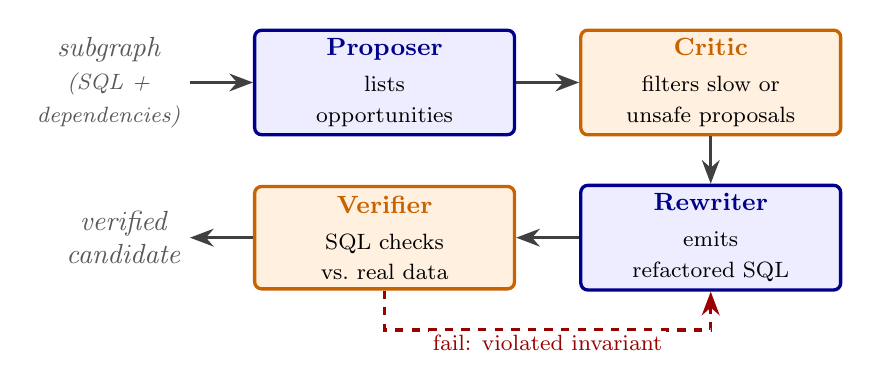
\begin{tikzpicture}[
    font=\small,
    node distance=6mm and 8mm,
    rolebase/.style={draw, rounded corners=2.5pt, very thick,
        minimum height=13mm, minimum width=33mm, align=center, inner sep=3pt, font=\small},
    gen/.style={rolebase, fill=blue!7,   draw=blue!55!black},
    chk/.style={rolebase, fill=orange!12, draw=orange!78!black},
    io/.style={align=center, font=\itshape, text=black!65},
    arrow/.style={-{Stealth[length=3mm]}, very thick, draw=black!75},
    backarrow/.style={-{Stealth[length=3mm]}, very thick, dashed, draw=red!60!black},
]
\node[io] (in) {subgraph\\\footnotesize(SQL +\\\footnotesize dependencies)};
\node[gen, right=of in]   (prop) {{\color{blue!55!black}\textbf{Proposer}}\\[2pt]\footnotesize lists\\\footnotesize opportunities};
\node[chk, right=of prop] (crit) {{\color{orange!78!black}\textbf{Critic}}\\[2pt]\footnotesize filters slow or\\\footnotesize unsafe proposals};
\node[gen, below=of crit] (rew)  {{\color{blue!55!black}\textbf{Rewriter}}\\[2pt]\footnotesize emits\\\footnotesize refactored SQL};
\node[chk, left=of rew]   (ver)  {{\color{orange!78!black}\textbf{Verifier}}\\[2pt]\footnotesize SQL checks\\\footnotesize vs.\ real data};
\node[io, left=of ver] (out) {verified\\candidate};
\draw[arrow] (in)   -- (prop);
\draw[arrow] (prop) -- (crit);
\draw[arrow] (crit) -- (rew);
\draw[arrow] (rew)  -- (ver);
\draw[arrow] (ver)  -- (out);
\draw[backarrow] (ver.south) -- ([yshift=-5mm]ver.south) -| (rew.south);
\node[font=\footnotesize, anchor=north, fill=white, inner sep=1.5pt]
  at ($(ver.south)!0.5!(rew.south) + (0,-5mm)$) {\color{red!60!black}fail: violated invariant};
\end{tikzpicture}%
}
% \inv
\caption{\dagsmith{}'s agentic refactoring loop. Four agents each fill one role: a \emph{proposer} and \emph{rewriter} (blue) generate, while a \emph{critic} and \emph{verifier} (amber) scrutinize. A failed equivalence check returns the violated invariant to the rewriter, which retries or reverts. }
\label{dag:fig:llm-refactoring}
\inv
\end{figure}

% \linc{Fonts are too small. Need to reference the figure in Section 3.2 when we overview the solution. Probably also want to change the color/shape a bit or add some symbols. Right now, the figure looks a bit plain.}




% \linc{Maybe we can say we use an agentic framework to address this with four separate agents? That might be a bit better framing I feel like.}
\dagsmith{} addresses all three with an agentic framework of four agents, each filling a single role  (Figure~\ref{dag:fig:llm-refactoring}): a \emph{proposer} reads the region and lists candidate optimizations, an adversarial \emph{critic} rejects proposals that would slow the pipeline or silently change its results, a \emph{rewriter} turns the survivors into concrete SQL, and a \emph{verifier} tests each rewrite against the warehouse's real data before it is trusted. Separating proposal from criticism keeps a single prompt from having to be both creative and skeptical, and grounding acceptance in real data rather than in the model's own assurance is what makes adopting LLM-written SQL safe.



\head{Proposal}
The first call ingests the subgraph's SQL and dependency edges and produces a domain-level reading of the region: a short semantic summary of each model and the end-to-end business question the subgraph answers. This reading is what lets later stages recognize equivalent computations written in dissimilar SQL. 
The call then outputs a list of \emph{opportunities}, each describing the work it would remove or shrink and how—proposals to be rewritten and checked by later agents.

\head{Filtering} A second call acts as an adversarial critic, going through the proposals and trying to break them. We keep this separate from proposal on purpose: a single prompt asked to both propose and doubt does neither well, and in practice the proposing voice often wins out. The critic looks for two failure modes. The first is a slowdown—a proposal that looks like reuse-driven savings but adds a write and a scan without cutting downstream work. The second is a correctness trap, of which Figure~\ref{dag:fig:critic-catch} shows one example: the proposal drops a join by reading a tag from a sibling deduplicated to one row per item, silently discarding the secondary tags the original join admitted. The critic returns one of three verdicts—\emph{approve}, \emph{reject}, or \emph{conditional}—where a conditional verdict records a data property the rewrite must satisfy, carried into the next stage.

\begin{figure}[!htbp]
\begin{minipage}[t]{0.48\linewidth}
\figsubheader{Original: join admits all tags}
\begin{lstlisting}[language=SQL]
SELECT i.item_id,
  MAX(CASE WHEN t.tag='A'
    THEN 1 ELSE 0 END) AS flag_a
FROM {{ ref('items') }} i
JOIN {{ ref('item_tags') }} t
  USING (item_id)
GROUP BY i.item_id
\end{lstlisting}
\end{minipage}
\hfill
\begin{minipage}[t]{0.48\linewidth}
\figsubheader{Proposal: drop join, read tag}
\begin{lstlisting}[language=SQL]
SELECT s.item_id,
  CASE WHEN s.tag='A'
    THEN 1 ELSE 0 END AS flag_a
FROM {{ ref('items_staged') }} s
-- items_staged keeps one tag/item;
-- secondary tags are silently lost
\end{lstlisting}
\end{minipage}
\inv
\caption{Correctness trap rejected by the critic. The original aggregates over all tags per item; the proposal reads from a sibling that has been deduplicated to one tag per item and silently drops the rest.}
\label{dag:fig:critic-catch}
\inv
\end{figure}

\head{Rewriting}
The opportunities that survive filtering, together with the analysis and the SQL of the affected nodes, go to a third call that produces concrete refactored SQL: it may rewrite nodes, mark nodes as removed, or introduce new shared nodes. Conditional opportunities carry their recorded constraints into this prompt. A node with consumers outside the subgraph may be rewritten internally but must produce identical output rows, since its contract with those consumers is fixed.


%A rewrite that passed filtering can still change the data, especially when one bundles several opportunities and a trap rejected on its own reappears nested inside a larger change: the staged-input shortcut of Figure~\ref{dag:fig:critic-catch}, for instance, can resurface inside a consolidated aggregation the critic approved on other grounds. \dagsmith{} therefore treats equivalence as an empirical question against real data. A fourth call, the \emph{correctness critic}, states for each adopted opportunity the data invariant that must hold for the rewrite to be safe and renders it as a SQL diagnostic that returns zero rows when the invariant holds and rows when it is violated. The diagnostics run against the target warehouse under a per-query byte cap; any returned row is a counterexample drawn from real data. Failed invariants are appended to the rewriting prompt, and the LLM must either find a distinctly different strategy that respects them or restore the original logic. The loop ends when the rewrite passes all diagnostics, the LLM reports no further distinct strategy, or a per-group attempt budget is exhausted, in which case the group reverts to its original SQL and contributes no candidate.
\head{Equivalence verification}
Filtering judges proposals one at a time, but the rewriter often bundles several into a single change—and a trap that the critic would have rejected on its own can slip back in once it is buried inside a larger rewrite. The grain-collapse shortcut of Figure~\ref{dag:fig:critic-catch}, for instance, can resurface inside a consolidated aggregation the critic approved on other grounds. 
Because a bundled rewrite can be wrong even after filtering, \dagsmith{} checks each one against real data. A fourth call, the \emph{verifier}, writes a check for every adopted opportunity: a SQL query that returns rows only when the rewrite has changed the data. These run against the target warehouse under a per-query byte cap, so any row that comes back is a real counterexample. When a check fails, the violated invariant goes back to the rewriter, which must either find a different strategy that respects it or revert to the original. The loop stops once every check passes, the LLM has no new strategy to try, or the per-group attempt budget runs out—in which case the group keeps its original SQL and contributes nothing. Because these checks run on the project's own data, they reject any divergence that data exposes but do not amount to a formal equivalence proof, so \dagsmith{} does not claim guaranteed correctness. Adopted rewrites are still meant for a final human check before deployment.

% \linc{Does this guarantee correctness? If not, do we have a manual verification stage? I think we could have a sentence to clarify this.}



\head{Model families and propagation}
A subgraph often contains a \emph{family} of near-duplicate models that apply the same operation to different data subsets, and running the full four-call sequence on each would be wasteful. \dagsmith{} instead runs it once on a representative and propagates the accepted rewrite to the rest with a lighter per-member call. Where a project has no family structure, the sequence runs over every model unchanged.












\subsection{Materialization Tuning}
\label{dag:sec:materialization}



\begin{figure}[t]
\centering
\resizebox{\columnwidth}{!}{%
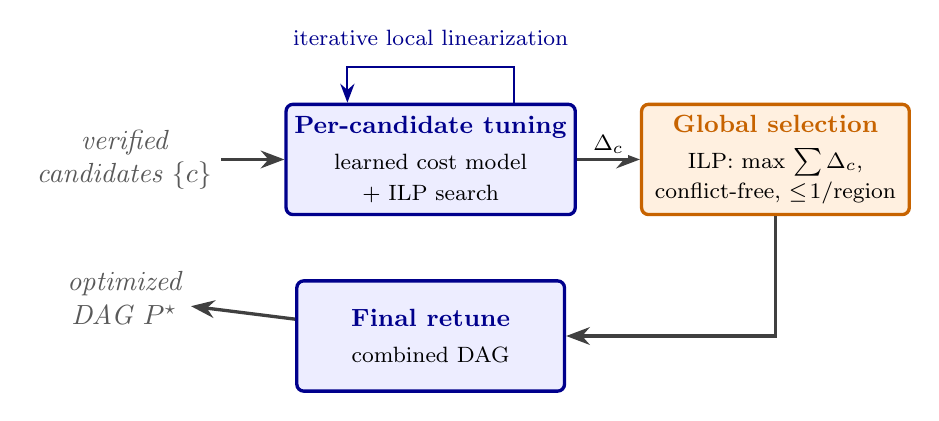
\begin{tikzpicture}[
    font=\small, node distance=8mm and 8mm,
    stagebase/.style={draw, rounded corners=2.5pt, very thick,
        minimum height=14mm, minimum width=34mm, align=center, inner sep=3pt, font=\small},
    tuneS/.style={stagebase, fill=blue!7,   draw=blue!55!black},
    selS/.style={stagebase, fill=orange!12, draw=orange!78!black},
    io/.style={align=center, font=\itshape, text=black!65},
    arrow/.style={-{Stealth[length=3mm]}, very thick, draw=black!75},
    looparrow/.style={-{Stealth[length=2.4mm]}, thick, draw=blue!55!black},
    albl/.style={font=\footnotesize, fill=white, inner sep=1.5pt},
]
\node[io] (in) {verified\\candidates $\{c\}$};
\node[tuneS, right=of in] (tune) {{\color{blue!55!black}\textbf{Per-candidate tuning}}\\[2pt]\footnotesize learned cost model\\\footnotesize $+$ ILP search};
\node[selS, right=of tune] (sel) {{\color{orange!78!black}\textbf{Global selection}}\\[2pt]\footnotesize ILP: max $\sum\Delta_c$,\\\footnotesize conflict-free, $\le\!1$/region};
\node[tuneS, below=of tune] (re) {{\color{blue!55!black}\textbf{Final retune}}\\[2pt]\footnotesize combined DAG};
\node[io, below=of in] (out) {optimized\\DAG $P^\star$};
\draw[arrow] (in)   -- (tune);
\draw[arrow] (tune) -- node[albl,above]{$\Delta_c$} (sel);
\draw[arrow] (sel.south) |- (re.east);
\draw[arrow] (re)   -- (out);
% elbow self-loop over the tuning box: iterative local linearization
\draw[looparrow] ([xshift=-8mm]tune.north east) -- ++(0,4.5mm) -| ([xshift=8mm]tune.north west);
\node[font=\footnotesize, anchor=south, inner sep=1pt, text=blue!55!black]
  at ([yshift=6.8mm]tune.north) {iterative local linearization};
\end{tikzpicture}%
}
% \inv
\caption{\dagsmith{}'s materialization tuning and global selection.}
\label{dag:fig:materialization}
\inv
\end{figure}

% \linc{Fonts are too small. Need to reference the figure in Section 3.3 when we overview the solution. Probably also want to change the color/shape a bit or add some symbols. Right now, the figure looks a bit plain.}

This stage realizes rewrite-materialization co-optimization. 
A refactoring's benefit cannot be determined in isolation: whether it helps depends on which of its nodes are stored as tables and which are inlined as views, and the best choice differs from one candidate to the next, so a candidate must be scored together with its own best materialization. This is especially important when a rewrite creates additional reusable output: the richer rewrite may be locally more expensive, but it can become beneficial when the output is materialized once and reused by enough downstream consumers. Even then, a second challenge remains: candidates overlap and cannot all be adopted at once, so they must be composed into a compatible set. This subsection addresses both (Figure~\ref{dag:fig:materialization}): tuning one candidate's materialization, then selecting a compatible set.





\head{Tuning one candidate}
To score a candidate, \dagsmith{} must find its best materialization: the assignment of each node to a table or a view that makes the whole pipeline cheapest to run, where \emph{cost} is 
the total slot time of executing the entire pipeline once.
% \linc{of the entire project? Or just one model?}
 That lowest cost becomes the candidate's score.

 Finding that assignment is hard because the table-or-view choice is not node-local: a view re-executes its SQL into every consumer that reads it, recursively through any view-parent. Flipping a node to a view therefore pushes its work downstream, coupling its cost to its descendants, so total cost is not a sum of per-node costs.
 
% Finding that assignment is hard because the table-or-view choice is not node-local. A table is a barrier: it is built once, and its consumers read its stored rows. A view is not: reading a view re-executes its SQL, expanding recursively through any view-parent until it reaches a table or source. Flipping a node from a table to a view therefore drops its own build cost but pushes its work, together with the view chain above it, into every consumer that reads it, once per consumer execution. A node's cost thus depends on how its ancestors are materialized, so the choices are coupled and total cost is not a sum of per-node costs. 


% \linc{This paragraph seems a bit abrupt. It doesn't connect either the paragraph above or below. What's the point of this paragraph? How is it relevant to the paragraph above and below?}
 
This coupling creates two challenges that \dagsmith{} handles in turn. 
% \linc{What are the two difficulties? The ``two reasons'' mentioned two paragraphs ago? Or something from the last paragraph?} 
The first is evaluation: scoring an assignment typically involves executing the pipeline, so \dagsmith{} instead uses a learned cost model to enable efficient approximation. Two robust (Huber~\cite{huber1964robust}) regressors, fit on instrumented runs of the original pipeline, predict each node's output cardinality and its slot time from structural features parsed off its compiled SQL, each conditioned on the predicted cardinalities of the node's parents.
Because a view's work folds into whoever reads it, \dagsmith{} accumulates each node's features up its view chain. A node's predicted cost then reflects the work it actually performs under the current table-or-view assignment, not just its own SQL. New nodes a refactoring introduces have no measured runs of their own and are predicted the same way, from their SQL features and their parents' predicted cardinalities.
% Because a view's work folds into whoever reads it, these features are accumulated along each view chain, so a node is priced on the work it performs under the assignment in question; new nodes a refactoring introduces, having no measurements of their own, are predicted the same way from their SQL and their parents' cardinality. 
% \linc{$\leftarrow$ The earlier sentence is difficult for me to parse.} 
The model only has to rank assignments within one project rather than predict absolute runtimes, so directional accuracy is enough, and the Huber loss keeps a handful of very large queries from dominating the fit.
 
The second is search: the best assignment must be found among exponentially many ($2^n$ for a candidate of $n$ nodes) possible solutions. \dagsmith{} navigates this with \textbf{iterative local linearization}~\cite{griffith1961slp,palaciosgomez1982slp}, a successive-approximation scheme that replaces the true nonlinear cost with a local linear surrogate, solves it, and re-linearizes at the result. Concretely, at iteration $k$, holding the current assignment $t^{(k)}$ fixed, \dagsmith{} uses the cost model to measure two local quantities: a baseline build cost $B^{(k)}_j$ for each node $j$ (its direct parents forced to tables) and an edge-local delta $U^{(k)}_{ij}$, the extra cost at $j$ when only parent $i$ is inlined as a view. Treating these as constants for the iteration, it solves a small ILP for $t^{(k+1)}$:
\begin{equation*}
\min_{t,\,y}\; \sum_{j \in V} t_j\, B^{(k)}_j \;+\; \sum_{i \to j \in E} y_{ij}\, U^{(k)}_{ij}, \qquad \text{s.t.}\quad y_{ij} = (1 - t_i) \wedge t_j,
\end{equation*}
where $y_{ij}$ is $1$ exactly when node $j$ is built and reads a view-parent $i$, and a trust-region cap on flips keeps each step where the coefficients hold. 
Because flipping a node changes the cardinalities its descendants see, $B$ and $U$ are recomputed after each move and the step repeated until the assignment stops changing; an effect the current coefficients miss, such as the cost of also flipping a sibling, then surfaces in the next round. This is what makes the coupled, nonlinear assignment tractable: instead of enumerating the $2^n$ assignments, each round solves one small ILP that weighs all nodes' table-or-view choices jointly under the current cost estimates, capturing interactions that a greedy, one-node-at-a-time search would miss. The search reaches a local optimum, not a global one, but this is safe: the original DAG is tuned by the same procedure and kept as a fallback, so an under-tuned candidate simply loses to it, costing at most a missed improvement rather than a regression below the original.



% Because flipping a node changes the cardinalities its descendants see, $B$ and $U$ are recomputed after each move and the step repeated until the assignment stops changing; an effect the current coefficients miss, such as the cost of also flipping a sibling, then surfaces in the next round. The loop converges to a local optimum rather than a global one, which is safe here. 
% Because the search minimizes cost, a worse assignment can only make a candidate look more expensive than its true best, never cheaper \linc{I don't really get the point of this local optimum discussion. I understand what you mean, but is this a good thing or a bad thing? Why do we want to discuss this?}; and a candidate is adopted only when it beats the original DAG, which is tuned by the same procedure and is always available as a fallback. A candidate the search shortchanges therefore loses to the original and is passed over, so imperfect search risks only a missed improvement, never a regression below the original. \linc{Okay, I think this is a really long and verbose discussion about even though the algorithm only converges to the local optimum, it never regresses. I think it should just be 1-2 sentences. Instead, you could briefly discuss the advantages of this algorithm for our problem. What it achieves for us, why it's better, etc.}





















\begin{comment}
    


\head{Tuning one candidate}
Finding a candidate's best materialization is hard because a node's materialization is not a local choice. A table acts as a barrier: it is built once, and its consumers read its stored rows. A view does not; a query that reads a view re-executes the view's SQL, expanding recursively through any parent that is itself a view until it reaches a table or source. Turning a node from table to view therefore removes its build cost but pushes its computation, along with the chain of views above it, into every query that reads it, once per consumer execution. A node's cost is set by a window of the DAG around it, and because those windows overlap, the choices are coupled: the marginal value of one decision depends on the rest of the assignment. Total cost is not a sum of per-node costs, which rules out tuning node by node, and the joint space is far too large to enumerate. \linc{What does this ``cost'' refer to? Where is it used? In general, I couldn't really follow the discussion here... I think we're missing the intuitive discussion (2-3 sentences) on at a high-level how our method works and why it's better. We use this learned cost model, but why? What does it do? Why it's better? We use this linear programming for each, but why? What does it do? Why it's better? Overall, what's our key methodology? You just need a few sentences to establish these, but without them, it's very difficult for me to follow the text below and understand why I'm reading it. You added this for Section 3.1 and 3.2, which helped a lot.}

Two different costs stand in the way, and \dagsmith{} addresses them separately. \linc{Are these two ``costs'' the same as the ``cost'' above? I'm confused...} The first is evaluation: scoring a configuration would normally mean executing it. A learned cost model, trained on instrumented runs of the original pipeline, predicts the cardinality and slot time of every node under a given assignment, which prices a whole configuration without running it; the new nodes a refactoring introduces, having no measurements, are predicted the same way from their SQL and their parents' cardinality. \linc{This ``cost model'' part is also a bit vague. What's the input of this model and how do we featurize it? What's the model algorithm (doesn't need the detailed equation, but we don't even now which ML model do we use... It's not going to be super accurate either, right? So what do we do if it's not accurate? We don't need all the details but we need some basic understanding of it.)}

The second is search. \linc{What is the goal of the search? Why do we need it? I don't think we have established it...} \dagsmith{} navigates the space with \textbf{iterative local linearization}, a successive-approximation scheme that replaces the true nonlinear cost with a local linear surrogate, solves it, and re-linearizes at the result. Concretely, at iteration $k$, holding the current assignment $t^{(k)}$ fixed, \dagsmith{} uses the cost model to measure two local quantities: a baseline build cost $B^{(k)}_j$ for each node $j$ (its direct parents forced to tables) and an edge-local delta $U^{(k)}_{ij}$, the extra cost at $j$ when only parent $i$ is inlined as a view. Treating these as constants for the iteration, it solves a small ILP for $t^{(k+1)}$:
\begin{equation*}
\min_{t,\,y}\; \sum_{j \in V} t_j\, B^{(k)}_j \;+\; \sum_{i \to j \in E} y_{ij}\, U^{(k)}_{ij}, \qquad \text{s.t.}\quad y_{ij} = (1 - t_i) \wedge t_j,
\end{equation*}
where $y_{ij}$ is $1$ exactly when node $j$ is built and reads a view-parent $i$, and a trust-region cap on flips keeps each step where the coefficients hold. Because flipping a node changes the cardinalities its descendants see, $B$ and $U$ are recomputed after each move and the step repeated until the assignment stops changing; an effect the current coefficients miss, such as the cost of also flipping a sibling, then surfaces in the next round. The loop converges to a local optimum rather than a global one. This is safe because the unrefactored DAG is itself scored as a baseline candidate: a candidate that lands on a poor assignment loses to it and is not adopted; imperfect search costs a missed opportunity, never a regression below the original.

\end{comment}







\head{Selecting a compatible set}
Tuning leaves each candidate with a single number, its \emph{delta}: how much cheaper the pipeline runs if that one refactoring is applied, with the original and the refactored version each at its own best materialization. Selection then decides which candidates to adopt. It would take all of them if it could, but two things get in the way. First, refactorings can conflict: two that rewrite, create, or remove the same model cannot both be applied. Second, the LLM sometimes proposes several alternative refactorings for the same region, and at most one of them may be chosen. \dagsmith{} therefore looks for the set of candidates with the largest total delta that has no conflicts and at most one variant per region, a small problem it hands to an off-the-shelf integer-program solver. One correction remains: because each delta was measured with the candidate tuned on its own, the best table-or-view choices for the chosen combination need not match any single candidate's, so \dagsmith{} retunes the combined project one final time, rerunning the same cost-model-guided search used for each candidate, now over the merged DAG with all selected refactorings in place. 
% \linc{How this ``retune'' is done? Maybe briefly explain this with one/half a sentence.}





\subsection{Frequency-Aware Optimization}
\label{dag:sec:frequency}

This stage realizes frequency-aware optimization. The stages so far treat each node's slot time as a fixed per-execution cost. In a recurring pipeline that is suboptimal: a node's real overhead is its per-run cost multiplied by how often it must actually run. Treating cost as per-execution therefore overvalues savings on rarely-run models and undervalues them on frequently-run ones. \dagsmith{} adds a frequency dimension to correct this. Effective frequencies are derived from the declared schedule at sink nodes and the observed update rates at source tables, propagated through the DAG, and applied at three layers;  the profile captures both how often inputs change and how often downstream outputs are consumed.  The first two layers leave the DAG structure intact, while the third feeds a new class of candidates back to candidate identification (Section~\ref{dag:sec:candidate-identification}).

\head{Layer 1: Frequency as cost weight}
Materialization tuning and selection (Section~\ref{dag:sec:materialization}) minimize cost as if every model ran at the same rate. \dagsmith{} reweights their cost-model inputs by each node's effective frequency before the decisions are made; nothing else about them changes.

\head{Layer 2: Reconciling scheduled and effective frequency}
A model's effective frequency is the rate at which it produces \emph{new} output, the slower of how often its consumers need fresh output ($f^{\text{demand}}_j$) and how often its inputs actually change ($f^{\text{data}}_j$):
\begin{equation*}
f_j = \min\!\big(f^{\text{demand}}_j,\; f^{\text{data}}_j\big).
\end{equation*}
Where the schedule fires faster than $f_j$, the model re-executes and reproduces the output it produced last time. \dagsmith{} flags such over-scheduled models and reduces their schedule to $f_j$. This changes neither SQL nor materialization, only the schedule, yet every redundant execution it removes is eliminated outright.

\head{Layer 3: Frequency-driven splitting hints}
The first two layers leave the DAG structure intact; the third changes it. When a model has parents that change at different rates, it inherits the fastest, so any work inside it that depends only on slow-changing parents is recomputed at the fast rate even though its inputs have not changed. \dagsmith{} identifies such models and emits the location to candidate identification as a hint, alongside the reuse and prune signals. The LLM then proposes a frequency split of the kind shown in Figure~\ref{dag:fig:strategy-c-sql-frequency}: the slow-side work is extracted into its own slow-cadence model and the original becomes a lightweight join, after which the candidate flows through the same filtering, rewriting, verification, and selection as any other.
